\documentclass[11pt]{article}

%\usepackage{xcolor} 
\usepackage{amssymb,amsfonts,amsmath,mathrsfs,mathtools}
\usepackage{graphicx, epsfig, epstopdf}
\usepackage{bm}
\usepackage[margin=1in,papersize={8.5in,11in}]{geometry}
\usepackage{times}
\usepackage{xcolor}
\usepackage{color}
\usepackage[pdftex, plainpages=false, colorlinks=true, linkcolor=blue, citecolor=blue, bookmarks=false]{hyperref}
\renewcommand{\thefootnote}{\fnsymbol{footnote}}

\newcommand{\vs}{\vspace{0.2cm}}
\newcommand{\noter}[1]{\textcolor{red}{{#1}}}
\newcommand{\noteb}[1]{\textcolor{blue}{{#1}}}

\makeatother

\def\hs{\hspace{1cm}}

\renewcommand{\baselinestretch}{1.4}

\title{Homework 2}
\author{Gomez - Math 19B}
\date{Due: Jan 26th, 2024}

\begin{document}

\maketitle

\noindent 
\normalsize
\raggedright

Exercises are taken from section 5.2 and 5.3 in the textbook. It is advised that those who haven't done any derivative calculus recently do some of the practice problems seen at the end of the assignment. 


\begin{enumerate}

\item 
5.2 Exercise 2: Draw a graph of the signed area represented by the integral and compute it using geometry. 
\[
\int_{-2}^{3} 2x + 4 dx
\]

\item 
5.2 Exercise 12: Calculate $\int_2^52x+1 dx$ in two ways: As the limit $\lim_{N\to\infty} R_N$ and using geometry.

\item 
5.2 Exercise 14: Refer to figure 15, Evaluate $\int_0^3 g(t) dt$ and $\int_3^5 g(t) dt$. 

\begin{center}
    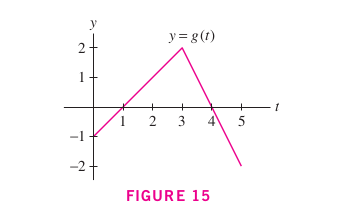
\includegraphics[width=.5\textwidth]{Sect 5.2 Exercise 14-15.png}
\end{center}

\item 
5.2 Exercise 41: Prove the following by computing the limit of right-endpoint approximations:

\[
\int_0^b x^3 dx = \frac{b^4}{4}
\]

\item 
5.2 Exercise 46: Use the formulas in the summary and equation (9) to evaluate the integral. 

\[
\int_0^1 2x^3 - x + 4 dx
\]
\item 
5.2 Exercise 64: Calculate the integral, assuming that f is an integrable function such that $\int_1^bf(x)dx = 1 - b^{-1}$ for all $b > 0$.
\[
\int_2^4f(x)dx
\]

\item 
5.3 Exercise 2: Sketch the region under the graph of the function and find its area using the Fundamental Theorem of Caluculus.

\[
    f(x) = 2x - x^2, [0, 2]
\]

\item 
5.3 Exercise 18: Evaluate the Integral using the Fundemental Theorem of Calculus. 
\[
    \int_{-1}^{1} 5x^4 - 6x^2 dx
\]

\item 
5.3 Exercise 48: Evaluate the integral in terms of the constants.
\[
\int_b^ax^4dx
\]
\end{enumerate}

\pagebreak


Derivative and Anti-Derivative Practice Problems: 

Definition: An \colorbox{yellow}{Anti-Derivative}, $F(x)$, of a function, $f(x)$, is any function such that, 
\[
\frac{d}{dx} [F(x)] = f(x)
\]
Anti-Derivatives are used to satisfy the Fundamental Theorem of Calculus in the following way,
\[
\int_a^bf(x)dx = F(b) - F(a)
\]
Thereby, having a more intimate knowledge of derivatives is an advantageous skill for computing integrals. 

Practice Problems (from section 3.8 in the textbook, all answers found in the back of the book)

\begin{enumerate}
\setcounter{enumi}{9}
\item 
3.8 Exercise 7.a: Calculate $\frac{d}{dx}cos(u(x))$ for the following choices of u(x):
\[
\text{a. } u(x) = 9 - x^2
\] 

\item 
3.8 Exercise 33: Use the chain rule to find the derivative
\[
    y = e^\frac{1}{x}
\]

\item 
3.8 Exercise 43: find the derivative using the appropriate rule or combination of rules. 
\[
y = \sqrt{\sin{x}\cos{x}}
\]

\item 
3.8 Exercise 47: find the derivative using the appropriate rule or combination of rules.
\[
y = (x + x^{-1})\sqrt{x + 1}
\]

\item 
3.8 Exercise 51: find the derivative using the appropriate rule or combination of rules.
\[
y = \tan^3{x} + \tan{x^3}
\]

\item 
3.8 Exercise 61: find the derivative using the appropriate rule or combination of rules.
\[
y = 4e^{-x} + 7e^{-2x}
\]

\item
3.8 Exercise 83: compute the indicated higher derivatives
\[
\frac{d^2}{dx^2}\sin{x^2}
\]
\end{enumerate}

%
\end{document}
%
%
